
\section{Modelo Identificado}


\begin{frame}{Observação}
\begin{itemize}
\item 2 horas 
\item 4.5 ciclos \quad$\sim$ 120 cubos montados e empilhados
\item 65 Entradas e Saídas
\item 19751 vetores registrados
\item 1321 vetores únicos
% cat 2019-05-10_1524NoTimeIOheader.csv | cut -d, -f1 --complement | sort -V | uniq | wc -l
\end{itemize}\end{frame}


\begin{frame}{Modelo Identificado}
\begin{itemize}
\item 2 caminhos 
\end{itemize}
\begin{figure}[H]
  \centering
  \includegraphics[width=0.5\textwidth]{results/all/states.pdf}
  \caption{Variação de número de estados em relação ao valor de $k$.}
    \label{fig:statesIdentOriginal}
  \end{figure}
  \note{
\begin{itemize}
\item usando o método de obtenção de caminhos foram encontrados 2 caminhos.
  \item pode ser explicado ao fato de ter comportamento concorrente no sistema,
    o que torna raro de voltarem ao mesmo estado inicial.
    \item mas também mostra que o sistema não foi observado por tempo
      suficiente. O que mostra que seria necessária a observação durante muitas
      horas e talvez dias.
  \item No gráfico vemos o aumento de estados com o valor de k
\end{itemize}
  }
\end{frame}

\begin{frame}{Modelo Identificado}
\begin{figure}[H]
  \centering
  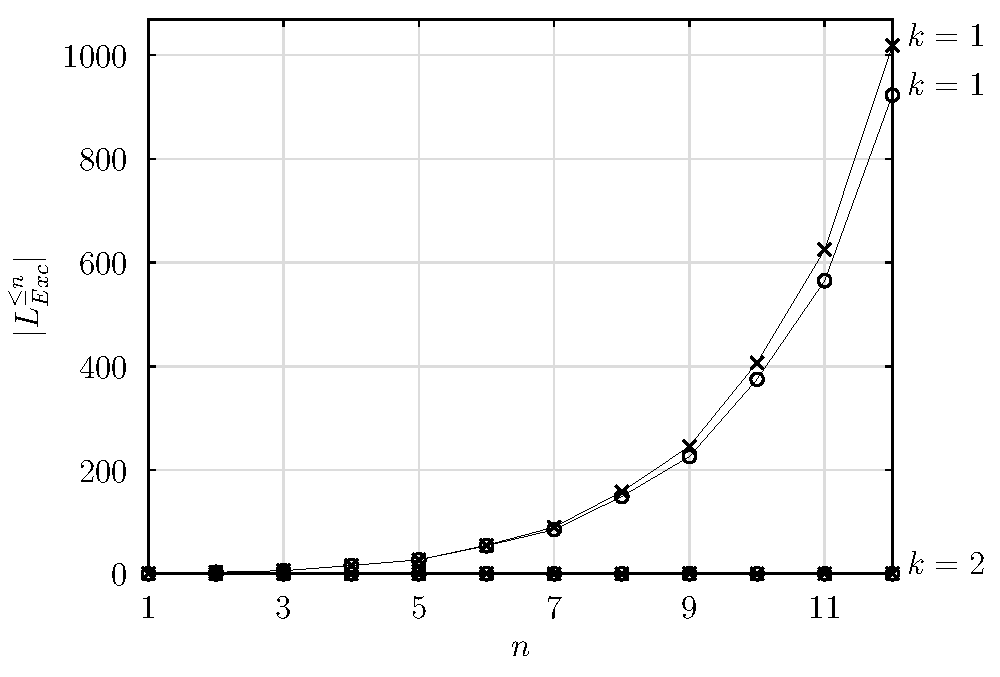
\includegraphics[width=0.5\textwidth]{results/all/exceedingLanguage-daoct-ndaao_k1-2_n12.pdf}
  \caption{Linguagens Excedentes - DAOCT (o), NDAAO ($\times$).}
    \label{fig:daoctNdaaoOriginal}
\end{figure}
  \note{
    \begin{itemize}
      \item Ndaao não usa os índices dos caminhos. Como poucos caminhos foram
        encontrados não aparenta uma diferennça tão significativa entre os
        modelos encontrados.
\item Comparando o modelo daoct encontrado com NDAAO, que é outro modelo de identificação, vemos que daoct tem menor
  linguagem excedente
\end{itemize}
  }
\end{frame}


\begin{frame}
\begin{itemize}
\item Verificar comportamento ao trocar vetor inicial \pause
\item Escolhido o vetor com maior incidência\pause
\item Descartam-se todos vetores anteriores a primeira incidência desse vetor
\end{itemize}
  \note{
\begin{itemize}
\item Fazer um experimento, trocar o vetor inicial para comparar o comportamento
\end{itemize}
  }
\end{frame}

\begin{frame}{Observação - Arquivo modificado}
\begin{itemize}
\item 19427 vetores registrados
\item 1294 vetores únicos
% cat 2019-05-10_1524NoTimeIOheader.csv | cut -d, -f1 --complement | sort -V | uniq | wc -l
\end{itemize}
  \note{
\begin{itemize}
\item diferença nos valores causado pela exclusão dos vetores anteriores a
  primeira incidência do vetor considerado inicial
\end{itemize}
  }
\end{frame}

\begin{frame}{Modelo Identificado - Arquivo Modificado}
\begin{itemize}
\item 80 caminhos 
\end{itemize}
\begin{figure}[H]
  \centering
  \includegraphics[width=0.5\textwidth]{results/all/best/states.pdf}
  \caption{Variação de número de estados em relação ao valor de $k$.}
    \label{fig:statesIdentOriginal}
\end{figure}
  \note{
\begin{itemize}
\item Utilizando o arquivo modificado encontraram-se 80 caminhos 
\item os estados possuem a mesma ordem de grandeza 
\end{itemize}
  }
\end{frame}

\begin{frame}{Modelo Identificado - Arquivo Modificado}
   \begin{figure}[ht]
       \begin{minipage}[b]{0.35\linewidth}
         \centering
    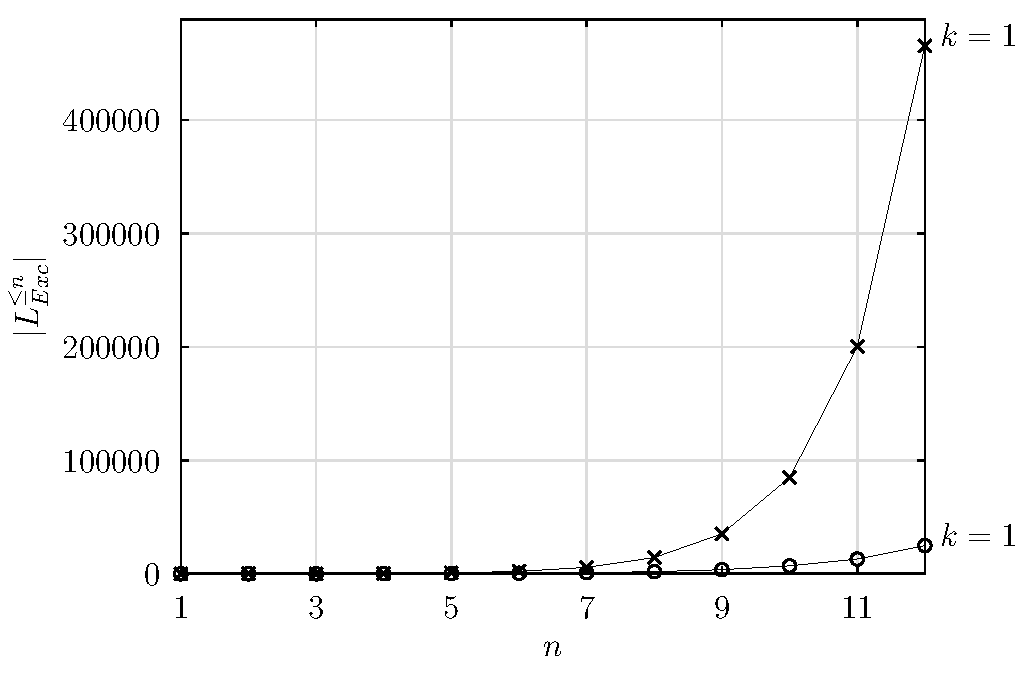
\includegraphics[width=\textwidth]{results/all/best/exceedingLanguage-daoct-ndaao_k1_n12.pdf}
\end{minipage}
       \begin{minipage}[b]{0.35\linewidth}
         \centering
    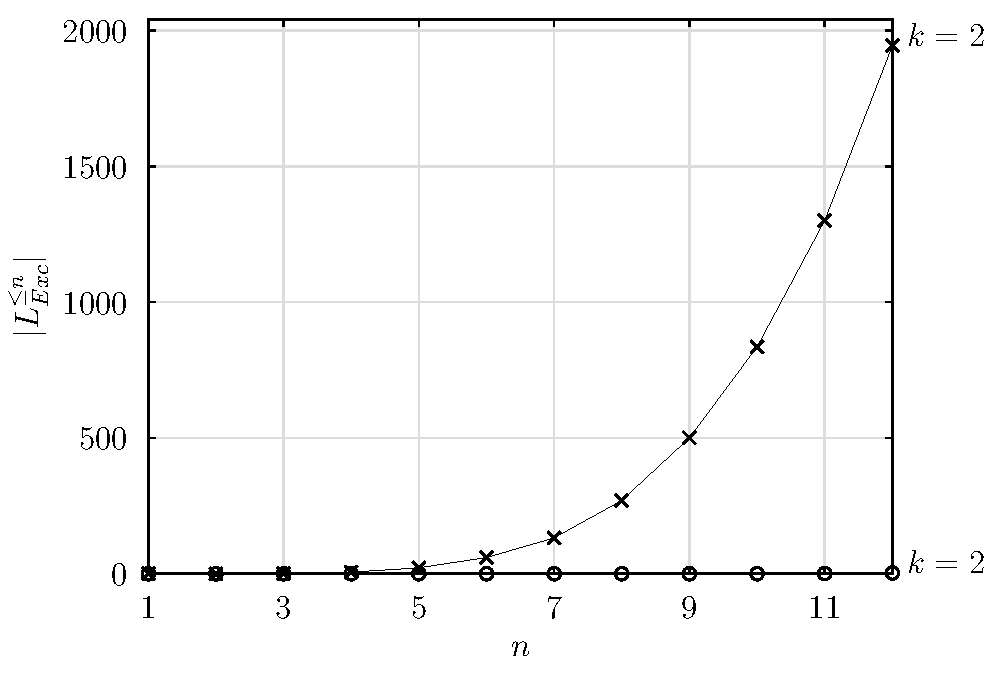
\includegraphics[width=\textwidth]{results/all/best/exceedingLanguage-daoct-ndaao_k2_n12.pdf}
       \end{minipage}
       \hspace{0.5cm}
       \begin{minipage}[b]{0.35\linewidth}
           \centering
    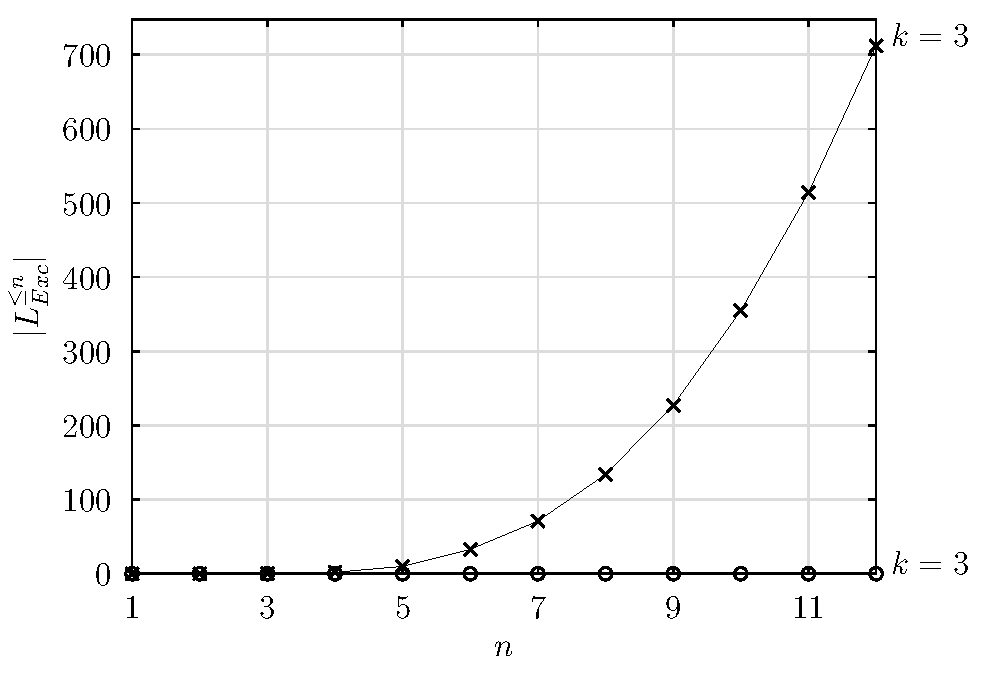
\includegraphics[width=\textwidth]{results/all/best/exceedingLanguage-daoct-ndaao_k3_n12.pdf}
       \end{minipage}
       \begin{minipage}[b]{0.35\linewidth}
           \centering
    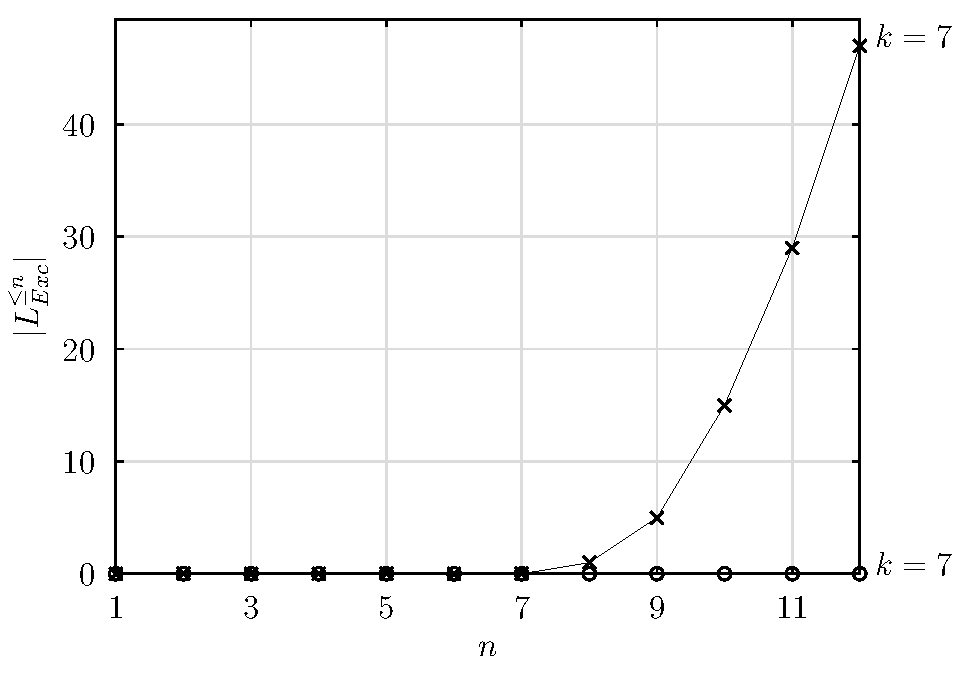
\includegraphics[width=\textwidth]{results/all/best/exceedingLanguage-daoct-ndaao_k7_n12.pdf}
       \end{minipage}
  \caption{Linguagens Excedentes - DAOCT (o), NDAAO ($\times$).}
   \end{figure}
  \note{
    \begin{itemize}
      \item Como dessa vez existem mais caminhos, a diferença por causa do uso
        dos índices de caminho do daoct aumenta.
\item para k=1 vemos a diferença consideravel: DAOCT está 50000 enquanto NDAAO
  está 400000
\item para k =3 enquanto NDAAO está acima de 700
\item embora a diferença seja melhor vista com mais caminhos, não
  necessariamente um modelo com mais caminhos represente melhor o sistema. Por
  isso vamos a um exemplo
\end{itemize}
  }
\end{frame}


\begin{frame}{Discussão Escolha Vetor inicial}
\begin{figure}[H]
  \centering
  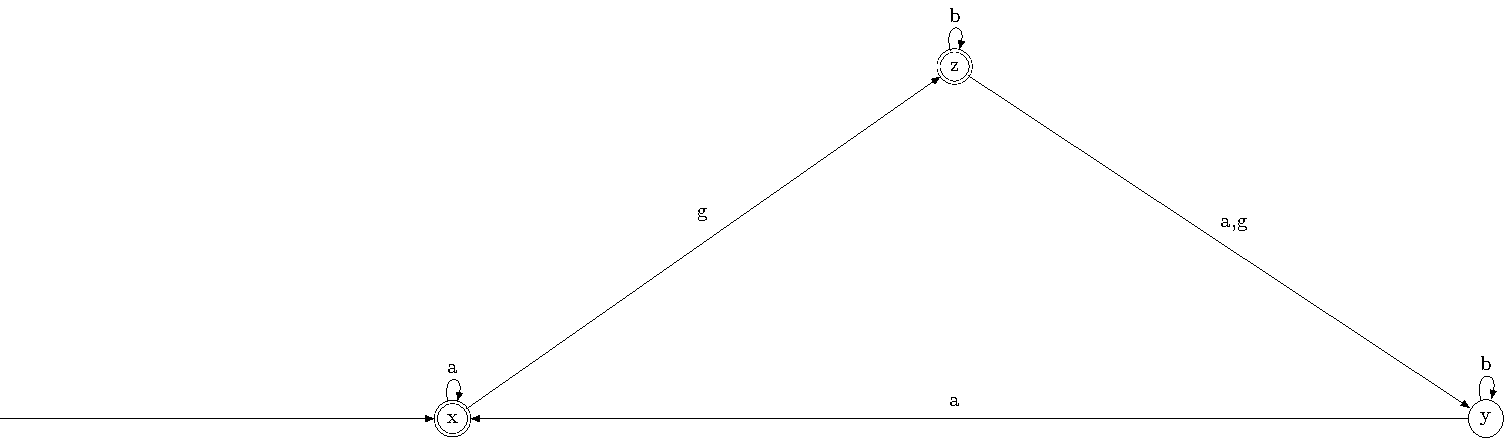
\includegraphics[width=.5\textwidth]{results/example/example}
  \caption{Exemplo de sistema a ser identificado.}
    \label{fig:schemeExConveyor}
\end{figure}
  \note{
\begin{itemize}
\item suponhamos um sistema formado por uma esteira e 3 sensores. Apenas uma
  caixa é colocada por vez na esteira. a esteira sempre ligada leva a caixa da
  esquerda para direita, ativando e desativando os sensores 1, 2 e 3 nessa
  ordem. Uma vez que a caixa sai da esteira, outra é colocada recomeçando o ciclo.
\end{itemize}
  }
\end{frame}

\begin{frame}{Discussão Escolha Vetor inicial}
\begin{align*}
  \label{motif}
{\only<2>{\color{gray}} {\only<4>{\color{blue}}\colvec{0\\0\\0}}\colvec{1\\0\\0}\colvec{0\\0\\0}\colvec{0\\1\\0}\colvec{0\\0\\0}\colvec{0\\0\\1} }
\only<1,2>{\colvec{0\\0\\0}\colvec{1\\0\\0}\colvec{0\\0\\0}\colvec{0\\1\\0}\colvec{0\\0\\0}\colvec{0\\0\\1}}
\end{align*}
  \note{
\begin{enumerate}
\item Digamos que a sequência de vetores de entrada e saídas foi a seguinte. 
\item a partir da sequência percebemos o seguinte padrão que se repete
\item então esse padrão corresponde a sequência mínima para identificar o
  sistema
  \item usando o método de obtenção de caminhos usamos o vetor 000 como vetor
    inicial e usando ele somos capazes de identificar o modelo seguinte
\end{enumerate}
  }
\end{frame}


\begin{frame}{Discussão Escolha Vetor inicial}
\begin{figure}[H]
  \centering
 \includegraphics[height=0.5\textheight]{results/example/examplek1NoArrows}
  \caption{Modelo identificado usando $\colvec{0&0&0}^T$ como vetor inicial, $k=1$.}
    \label{fig:exampleCol000k1}
\end{figure}
  \note{
\begin{itemize}
\item Nesse modelo usando 000 vemos que 3 caminhos são encontrados
\item Porém não vemos que existe uma ordem de ocorrência dos eventos, como
  mostrado na definição do sistema 3 pode acontecer antes de 1 e o modelo vai
  identificar como correto.
\end{itemize}
  }
\end{frame}

\begin{frame}{Discussão Escolha Vetor inicial}
  \note{
\begin{itemize}
\item como é cíclico podemos pegar o primeiro vetor e colocar como o último
\item e escolhemos agora 100 como vetor inicial
\end{itemize}
  }
\begin{align*}
\onslide<1>{\colvec{0\\0\\0}}{\only<3>{\color{blue}}\colvec{1\\0\\0}}\colvec{0\\0\\0}\colvec{0\\1\\0}\colvec{0\\0\\0}\colvec{0\\0\\1}\onslide<2->{\colvec{0\\0\\0}}
\end{align*}
\end{frame}

\begin{frame}{Discussão Escolha Vetor inicial}
\begin{figure}[H]
  \centering
  \includegraphics{results/example/example1k1NoArrows}
  \caption{Modelo identificado usando $\colvec{1&0&0}^T$ como vetor inicial, $k=1$}
    \label{fig:exampleCol100k1}
\end{figure}
  \note{
\begin{itemize}
\item Nesse modelo já vemos que há a ideia da ordem dos eventos, eventos 2 e 3
  só ocorrem apos 1.
\item Porém não vemos que o 2 precisa acontecer antes do 3. Nesse caso, se
  usarmos um k maior.
\end{itemize}
  }
\end{frame}

\begin{frame}{Discussão Escolha Vetor inicial}
\begin{figure}[H]
  \centering
  \includegraphics[width=\textwidth]{results/example/example1k2NoArrows}
  \caption{Modelo identificado usando $\colvec{1&0&0}^T$ como vetor inicial, $k=2$.}
    \label{fig:exampleCol100k2}
  \end{figure}
  \note{
\begin{itemize}
\item Vemos a ordem descrita no exemplo
\item Esse modelo representa fielmente o descrito no exemplo.
  \item podemos ver que o modelo depende de bons caminhos. E que
    se não conhecemos é difícil julgar se os caminhos obtidos são de fato bons
    ou não.
\end{itemize}
  }
\end{frame}



%%% Local Variables:
%%% mode: latex
%%% TeX-master: "../presentation"
%%% End: